\documentclass[10pt, aspectratio=169]{beamer}

% --- Theme & Colors ---
\usetheme{metropolis}
\setbeamercolor{background canvas}{bg=white}
\setbeamercolor{normal text}{fg=black!90}
\setbeamercolor{frametitle}{bg=white, fg=blue!50!black}
\setbeamercolor{progress bar}{fg=blue!60!black}
\setbeamercolor{itemize item}{fg=blue!60!black}

% --- Packages ---
\usepackage{tikz}
\usetikzlibrary{shapes, arrows, positioning, calc, shadows, fit, backgrounds, decorations.pathmorphing}
\usepackage{booktabs}
\usepackage{amsmath}
\usepackage{graphicx}
\usepackage{mwe} % For placeholder images
\usepackage{fontawesome5}
\usepackage{tcolorbox}

% --- Meta Data ---
\title{Water Network Leak Detection System}
\subtitle{A Digital Twin \& Multi-Agent Approach}
\author{AI Master's Cohort}
\date{\today}
\institute{Advanced AI for Critical Infrastructure}

\begin{document}

% --- Title Slide ---
\maketitle

% --- Slide 1: The Problem ---
\begin{frame}{The "Boring" Problem with Huge Consequences}
    \begin{columns}
        \column{0.6\textwidth}
        \textbf{Water Distribution Networks are leaky buckets.}
        \begin{itemize}
            \item \textbf{Non-Revenue Water:} Utilities often lose 20-30\% of total supply before it reaches the customer.
            \item \textbf{The Old Way:} Relying on angry customer phone calls or expensive, periodic acoustic surveys.
            \item \textbf{The Risk:} Infrastructure damage, service disruption, and massive financial waste.
        \end{itemize}
        \vspace{1em}
        \emph{We need a system that sleeps with one eye open.}
        
        \column{0.4\textwidth}
        \begin{center}
             % Placeholder image for broken pipe
             \includegraphics[width=\textwidth, height=6cm, keepaspectratio]{images/bucharest.png} 
             \small{\\ \textit{Figure: The reality of infrastructure damage.}}
        \end{center}
    \end{columns}
\end{frame}

% --- Slide 2: The Solution Overview ---
\begin{frame}{The Solution: Digital Twins meet AI Agents}
    We built a \textbf{Digital Twin} platform that combines hydraulic simulation with a \textbf{Multi-Agent System (MAS)}.
    \begin{enumerate}
        \item \textbf{Digital Twin:} A virtual replica using WNTR (Water Network Tool for Resilience) to simulate physics in real-time.
        \item \textbf{Distributed Intelligence:} Instead of one central brain, we use a team of agents.
        \item \textbf{Adaptive Math:} Statistical anomaly detection that learns "normal" over time.
    \end{enumerate}
\end{frame}

% --- Slide 3: The L-Town Network Topology ---
\begin{frame}{The Test Bed: L-Town Water Distribution Network}
    \begin{columns}
        % Left Column: The Data
        \column{0.6\textwidth}
            \textbf{1. The Physical Network (v1.2)}
            \begin{itemize}
                \item \textbf{Scale:} Real-world benchmark from battLeDIM 2020.
                \item \textbf{Assets:} 782 Junctions, $\sim$900 Pipes, 1 Tank.
                \item \textbf{Hydraulics:} Complex terrain with 2m--100m elevation changes and 3 Pressure Reducing Valves (PRVs).
            \end{itemize}
            
            \vspace{1em}
            \textbf{2. The Sensor Layer (Sparse)}
            \begin{itemize}
                \item \textbf{Pressure:} 33 Sensors (Only \textbf{4.2\%} coverage).
                \item \textbf{Flow:} 82 AMR Meters ($\sim$10.5\% coverage).
                \item \textbf{The Challenge:} We must localize leaks using data from less than 5\% of the network.
            \end{itemize}

        % Right Column: The Visuals
        \column{0.4\textwidth}
            \begin{center}
                % Placeholder for L-Town Map
                \includegraphics[width=\textwidth, height=4.5cm, keepaspectratio]{images/l_town_topo.jpg}
                \small{\\ \textit{Figure: L-Town Topology}}
            \end{center}
            \vspace{0.2em}
            \begin{block}{Why L-Town?}
                It combines realistic data sparsity with standard EPANET physics, making results verifiable.
            \end{block}
    \end{columns}
\end{frame}

% --- Slide 4: System Architecture (Diagram) ---
\begin{frame}{System Architecture: The 5-Layer Cake}
    \centering
    \resizebox{0.6\textwidth}{!}{
    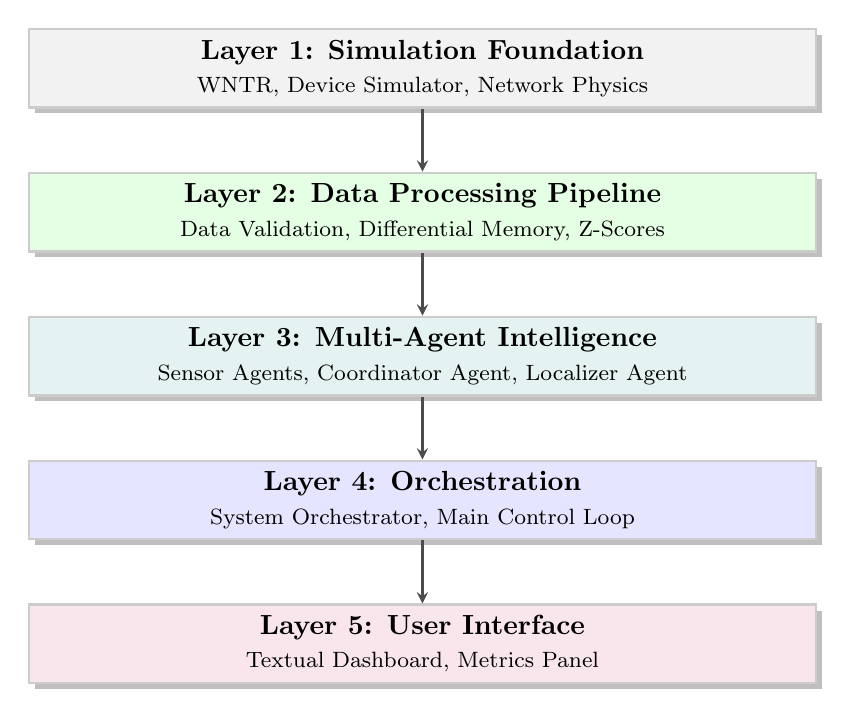
\begin{tikzpicture}[
        node distance=0.8cm,
        layer/.style={rectangle, draw=gray!40, thick, minimum width=10cm, minimum height=1cm, align=center, fill=blue!5, text=black, drop shadow},
        arrow/.style={->, >=stealth, thick, black!70}
    ]
        \node[layer, fill=gray!10] (l1) {\textbf{Layer 1: Simulation Foundation}\\ \footnotesize{WNTR, Device Simulator, Network Physics}};
        \node[layer, below=of l1, fill=green!10] (l2) {\textbf{Layer 2: Data Processing Pipeline}\\ \footnotesize{Data Validation, Differential Memory, Z-Scores}};
        \node[layer, below=of l2, fill=teal!10] (l3) {\textbf{Layer 3: Multi-Agent Intelligence}\\ \footnotesize{Sensor Agents, Coordinator Agent, Localizer Agent}};
        \node[layer, below=of l3, fill=blue!10] (l4) {\textbf{Layer 4: Orchestration}\\ \footnotesize{System Orchestrator, Main Control Loop}};
        \node[layer, below=of l4, fill=purple!10] (l5) {\textbf{Layer 5: User Interface}\\ \footnotesize{Textual Dashboard, Metrics Panel}};
        \draw[arrow] (l1) -- (l2);
        \draw[arrow] (l2) -- (l3);
        \draw[arrow] (l3) -- (l4);
        \draw[arrow] (l4) -- (l5);
    \end{tikzpicture}
    }
\end{frame}

% --- Slide 5: The Simulation Layer ---
\begin{frame}{Layer 1: The "Matrix" for Water}
    Before we deploy AI, we need a world.
    
    \begin{itemize}
        \item \textbf{Network Simulator:} Loads EPANET files (standard hydraulic models) and simulates pressure/flow in real-time.
        \item \textbf{Device Simulator:} We don't just simulate water; we simulate the \textit{sensors}.
        \begin{itemize}
            \item Adds realistic noise.
            \item Simulates battery drain (Idle: 0.5mW vs Sampling: 50mW).
            \item Can simulate sensor corruption or failures.
        \end{itemize}
    \end{itemize}
    \begin{block}{Why?}
        It allows us to inject leaks safely (programmatically) without flooding the basement.
    \end{block}
\end{frame}

% --- Slide 6: The AI Squad (Multi-Agent System) ---
\begin{frame}{The AI Squad: Meet the Agents}
    The intelligence is distributed across three types of agents:
    \vspace{1em}

    \begin{columns}[t]
        
        % --- Agent 1: Sensor (Blue Theme) ---
        \column{0.32\textwidth}
        \begin{tcolorbox}[colback=blue!5!white, colframe=blue!75!black, title=\centering \faEye \ \textbf{Sensor Agent}]
            \centering
            \footnotesize \emph{"The Watchman"}
            \vspace{0.5em}
            \begin{itemize}
                \item Lives at every node.
                \item Monitors pressure.
                \item \textbf{Gossip Check}.
            \end{itemize}
        \end{tcolorbox}

        % --- Agent 2: Coordinator (Teal/Green Theme) ---
        \column{0.32\textwidth}
        \begin{tcolorbox}[colback=teal!5!white, colframe=teal!75!black, title=\centering \faUserTie \ \textbf{Coordinator}]
            \centering
            \footnotesize \emph{"The Manager"}
            \vspace{0.5em}
            \begin{itemize}
                \item Aggregates alerts.
                \item Opens cases.
                \item Requests localization.
            \end{itemize}
        \end{tcolorbox}

        % --- Agent 3: Localizer (Red Theme) ---
        \column{0.32\textwidth}
        \begin{tcolorbox}[colback=red!5!white, colframe=red!75!black, title=\centering \faSearchLocation \ \textbf{Localizer}]
            \centering
            \footnotesize \emph{"The Detective"}
            \vspace{0.5em}
            \begin{itemize}
                \item Triangulates position.
                \item Graph algorithms.
                \item Ranks candidates.
            \end{itemize}
        \end{tcolorbox}

    \end{columns}
\end{frame}

% --- Slide 7: How Detection Works (Visualized) ---
\begin{frame}{The Math: Z-Scores \& Differential Memory}
    \begin{columns}
        % Left Column: The Equations
        \column{0.5\textwidth}
            \textbf{1. Adaptive Baseline \& Differential Memory}
            \small{Learns "normal" behavior while retaining hydraulic offsets for historical context.}
            $$ \mu_{t+1} = \mu_{t} + \alpha(x_{t} - \mu_{t}) $$
            \vspace{1em}
            
            \textbf{2. Anomaly Detection (Z-Score)}
            \small{Triggers if reading deviates $>3.0\sigma$ from mean.}
            $$ z = \frac{x - \mu}{\sigma} $$
        
        % Right Column: The Visuals
        \column{0.5\textwidth}
            \centering
            % Visual 1: EMA Chart
            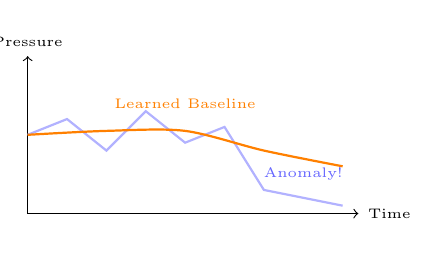
\begin{tikzpicture}[scale=1, trim left=0cm]
                \draw[->] (0,0) -- (4.2,0) node[right] {\tiny Time};
                \draw[->] (0,0) -- (0,2) node[above] {\tiny Pressure};
                % Noisy Data
                \draw[blue!30, thick] plot coordinates {(0,1) (0.5,1.2) (1,0.8) (1.5,1.3) (2,0.9) (2.5,1.1) (3,0.3) (3.5,0.2) (4,0.1)};
                % Smooth EMA
                \draw[orange, thick, smooth] plot coordinates {(0,1) (1,1.05) (2,1.05) (3,0.8) (4,0.6)};
                \node[orange, font=\tiny] at (2, 1.4) {Learned Baseline};
                \node[blue!60, font=\tiny] at (3.5, 0.5) {Anomaly!};
            \end{tikzpicture}
            
            \vspace{6.5em}
            
            % Visual 2: Bell Curve
            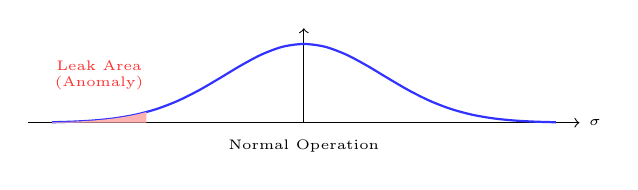
\begin{tikzpicture}[scale=1]
                    % Axis
                    \draw[->] (-3.5,0) -- (3.5,0) node[right] {\tiny $\sigma$};
                    \draw[->] (0,0) -- (0,1.2);
                
                    % The Bell Curve
                    \draw[domain=-3.2:3.2, smooth, variable=\x, blue!80, thick] plot ({\x}, {exp(-0.5*\x*\x)});
                
                    % The "Leak Area" (Exaggerated for visibility)
                    % We fill from -3.2 to -2.0 so the shape is large enough to see
                    \fill[red!30] (-3.2,0) -- plot[domain=-3.2:-2.0] (\x, {exp(-0.5*\x*\x)}) -- (-2.0,0) -- cycle;
                
                    % Labels
                    \node[font=\tiny, red!80, align=center] at (-2.6, 0.6) {Leak Area\\(Anomaly)};
                    \node[font=\tiny, black] at (0, -0.3) {Normal Operation};
                \end{tikzpicture}
    \end{columns}
\end{frame}

% --- Slide 8: Localization (Visualized) ---
\begin{frame}{The Math: Finding the Source (Localization)}
    \begin{columns}
        % Left Column: The Equation and Logic
        \column{0.55\textwidth}
            \textbf{Distance-Weighted Triangulation}
            \vspace{0.5em}
            
            We calculate a "Leak Likelihood Score" for every node $n$:
            
            \begin{equation*}
                \text{Score}(n) = \sum_{i \in \text{Sensors}} \frac{\textcolor{red}{\mathbf{w_i}}}{\textcolor{gray}{d_0} + \textcolor{blue}{\mathbf{d(n, s_i)}}}
            \end{equation*}
            
            \vspace{1em}
            \textbf{The Variables:}
            \begin{itemize}
                \item \textcolor{red}{$\mathbf{w_i}$}: \textbf{Signal Strength}. (Z-Score magnitude).
                \item \textcolor{blue}{$\mathbf{d(n, s_i)}$}: \textbf{Pipe Distance}. Shortest path in network.
                \item \textcolor{gray}{$\mathbf{d_0}$}: \textbf{Smoothing}. Constant (100) to avoid $\div 0$.
            \end{itemize}

        % Right Column: The Visual Intuition
        \column{0.45\textwidth}
            \centering
            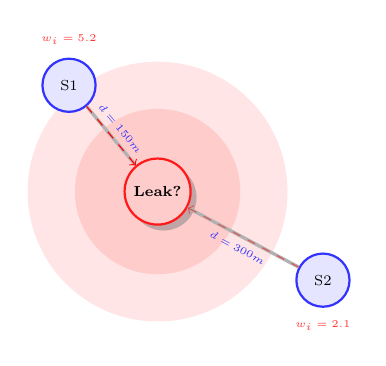
\begin{tikzpicture}[
    scale=0.75, transform shape,
    node distance=2cm,
    pipe/.style={draw, very thick, gray!60},
    sensor/.style={circle, draw=blue!80, fill=blue!10, thick, minimum size=0.9cm, align=center, font=\scriptsize},
    leak/.style={circle, draw=red!90, fill=red!20, thick, minimum size=0.9cm, drop shadow, font=\bfseries\scriptsize},
    junction/.style={circle, draw=gray, fill=white, minimum size=0.3cm}
]
    % Heat rings
    \fill[red!10] (1, -1) circle (2.2cm);
    \fill[red!20] (1, -1) circle (1.4cm);

    % Nodes
    \node[leak] (L) at (1, -1) {Leak?};
    
    % --- ADJUSTED COORDINATES ---
    % S1: Middle ground. Enough space for text, but compact.
    \node[sensor] (S1) at (-0.5, 0.8) {S1}; 
    
    % S2: Pushed out just enough to look longer than S1
    \node[sensor] (S2) at (3.8, -2.5) {S2}; 
    % ----------------------------
    
    % Edges
    \draw[pipe] (S1) -- node[above, sloped, text=blue!80] {\tiny $d=150m$} (L);
    \draw[pipe] (L) -- node[below, sloped, text=blue!80] {\tiny $d=300m$} (S2);
    
    % Weights
    \node[text=red!80, above=0.1cm of S1, font=\bfseries\tiny] {$w_i=5.2$};
    \node[text=red!80, below=0.1cm of S2, font=\bfseries\tiny] {$w_i=2.1$};
    
    % Pull vectors
    \draw[->, red, dashed] (S1) -- (L);
    \draw[->, red, dashed, opacity=0.5] (S2) -- (L);
\end{tikzpicture}
            
            \vspace{0.5em}
            \small{\textit{\textbf{Intuition:} The leak is "pulled" towards sensors with the highest anomaly scores.}}
    \end{columns}
\end{frame}

% --- Slide 9: The Dashboard (TUI) ---
\begin{frame}{The Interface: Terminal UI}
    We built a "Hacker-style" interface using Python's \texttt{Textual} framework.
    It visualizes real-time metrics, active alerts, and agent states.
    \begin{center}
        % Placeholder for Dashboard UI
        \includegraphics[width=0.95\textwidth, height=5.5cm, keepaspectratio]{images/tui.png}
        \\ \small{\textit{Screenshot: The System Dashboard running in a terminal.}}
    \end{center}
\end{frame}

% --- Slide 10: Workflow Diagram ---
\begin{frame}{Workflow: From Leak to Detection}
    \centering
    \resizebox{0.95\textwidth}{!}{
    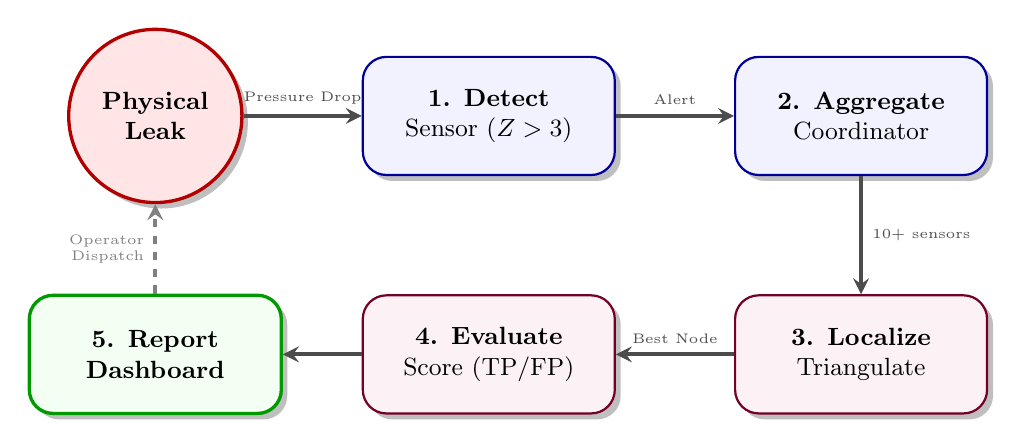
\begin{tikzpicture}[
        node distance=1.5cm and 1.5cm,
        % --- Styles ---
        startnode/.style={circle, draw=red!70!black, fill=red!10, very thick, minimum size=2.2cm, align=center, drop shadow, font=\small\bfseries},
        process/.style={rectangle, draw=blue!60!black, fill=blue!5, thick, minimum width=3.2cm, minimum height=1.5cm, rounded corners=3mm, align=center, drop shadow, font=\small},
        decision/.style={rectangle, draw=purple!60!black, fill=purple!5, thick, minimum width=3.2cm, minimum height=1.5cm, rounded corners=3mm, align=center, drop shadow, font=\small},
        endnode/.style={rectangle, draw=green!60!black, fill=green!5, very thick, minimum width=3.2cm, minimum height=1.5cm, rounded corners=3mm, align=center, drop shadow, font=\small\bfseries},
        % --- Line Styles ---
        line/.style={draw, ->, >=stealth, color=black!70, line width=1.5pt},
        dashed_line/.style={draw, ->, >=stealth, dashed, color=gray, line width=1.5pt},
        label/.style={font=\scriptsize, color=blue!60!black, midway}
    ]
       
        % --- Top Row (The Leak & Detection) ---
        \node[startnode] (leak) {Physical\\Leak};
        \node[process, right=of leak] (detect) {\textbf{1. Detect}\\Sensor ($Z > 3$)};
        \node[process, right=of detect] (aggregate) {\textbf{2. Aggregate}\\Coordinator};
       
        % --- Bottom Row (Localization & Report) ---
        \node[decision, below=of aggregate] (localize) {\textbf{3. Localize}\\Triangulate};
        
        \node[decision] at (detect |- localize) (evaluate) {\textbf{4. Evaluate}\\Score (TP/FP)};
        
        \node[endnode] at (leak |- localize) (report) {\textbf{5. Report}\\Dashboard};

        % --- Main Flow Connections ---
        \draw[line] (leak) -- node[above, font=\tiny] {Pressure Drop} (detect);
        \draw[line] (detect) -- node[above, font=\tiny] {Alert} (aggregate);
        \draw[line] (aggregate) -- node[right, font=\tiny] {10+ sensors} (localize);
        \draw[line] (localize) -- node[above, font=\tiny] {Best Node} (evaluate);
        \draw[line] (evaluate) -- (report);

        % --- Feedback Loop (Operator Action) ---
        \draw[dashed_line] (report.north) -- node[left, font=\tiny, text=gray, align=right] {Operator\\Dispatch} (leak.south);

    \end{tikzpicture}
    }
    \vspace{0.5em}
    \small{\textit{Evaluation scores detections against ground truth for metrics only, agents never see the answer.}}
\end{frame}

% --- Slide 10b: Investigation Sequence Diagram ---
\begin{frame}{Investigation Lifecycle: The Detailed Flow}
    \centering
    \resizebox{0.92\textwidth}{!}{
    \begin{tikzpicture}[
        node distance=0.6cm and 0.8cm,
        agent/.style={rectangle, draw=#1!70!black, fill=#1!10, thick, minimum width=2cm, minimum height=0.8cm, align=center, font=\footnotesize\bfseries},
        action/.style={rectangle, draw=gray!50, fill=white, minimum width=2.5cm, minimum height=0.5cm, align=center, font=\tiny, rounded corners=2mm},
        message/.style={->, >=stealth, thick, #1},
        timeline/.style={draw, gray!30, dashed},
        phase/.style={rectangle, draw=#1!60, fill=#1!5, rounded corners=3mm, minimum width=2.8cm, minimum height=0.45cm, font=\tiny\bfseries, align=center}
    ]
        % === AGENT HEADERS (Top Row) ===
        \node[agent=red] (leak) at (0, 0) {\faWater\ Leak};
        \node[agent=blue] (s1) at (3, 0) {\faEye\ Sensor 1};
        \node[agent=blue] (s2) at (5.5, 0) {\faEye\ Sensor 2};
        \node[agent=blue] (sn) at (8, 0) {\faEye\ Sensor N};
        \node[agent=teal] (coord) at (11.5, 0) {\faUserTie\ Coordinator};
        \node[agent=orange] (local) at (15, 0) {\faSearchLocation\ Localizer};
        
        % === VERTICAL TIMELINES ===
        \foreach \x in {0, 3, 5.5, 8, 11.5, 15} {
            \draw[timeline] (\x, -0.5) -- (\x, -7.8);
        }
        
        % === PHASE 1: Detection ===
        \node[phase=red] at (-2.2, -1) {PHASE 1\\Detection};
        
        % Leak causes pressure drop (wavy lines for physics)
        \draw[message=red!70, decorate, decoration={snake, amplitude=0.8mm, segment length=3mm}] (0, -0.9) -- node[above, font=\tiny, text=red!70] {$\Delta P$} (3, -1.3);
        \draw[message=red!70, decorate, decoration={snake, amplitude=0.8mm, segment length=3mm}] (0, -1.1) -- (5.5, -1.6);
        \draw[message=red!70, decorate, decoration={snake, amplitude=0.8mm, segment length=3mm}] (0, -1.3) -- (8, -1.9);
        
        % Sensors compute Z-score
        \node[action] at (3, -1.9) {$Z = 4.2$};
        \node[action] at (5.5, -2.2) {$Z = 3.8$};
        \node[action] at (8, -2.5) {$Z = 3.1$};
        
        % === PHASE 2: Alert Aggregation ===
        \node[phase=blue] at (-2.2, -3.2) {PHASE 2\\Aggregation};
        
        % Sensors send alerts to coordinator
        \draw[message=blue!70] (3, -2.4) -- node[above, sloped, font=\tiny] {ALERT} (11.5, -3.0);
        \draw[message=blue!70] (5.5, -2.7) -- node[above, sloped, font=\tiny] {ALERT} (11.5, -3.3);
        \draw[message=blue!70] (8, -3.0) -- node[above, sloped, font=\tiny] {ALERT} (11.5, -3.6);
        
        % Coordinator decision box
        \node[action, fill=teal!10, minimum width=3cm] at (11.5, -4.1) {$\geq 3$ sensors? \textcolor{green!60!black}{\faCheck}};
        \node[action, fill=teal!15, minimum width=3cm] at (11.5, -4.65) {\textbf{Open INV-0001}};
        
        % === PHASE 3: Localization ===
        \node[phase=teal] at (-2.2, -5.3) {PHASE 3\\Localization};
        
        % More alerts indicator
        \node[font=\tiny, gray, align=center] at (5.5, -5.0) {$\cdots$ more alerts arrive $\cdots$\\(until 10+ sensors)};
        
        % Coordinator requests localization
        \draw[message=teal!70, very thick] (11.5, -5.3) -- node[above, font=\tiny\bfseries] {LOCALIZE\_REQ} (15, -5.3);
        
        % Localizer computes
        \node[action, fill=orange!10] at (15, -5.85) {Triangulate};
        \node[action, fill=orange!15] at (15, -6.4) {$\sum \frac{w_i}{100+d_i}$};
        
        % Result back
        \draw[message=orange!70, very thick] (15, -6.9) -- node[above, font=\tiny\bfseries] {RESULT: n458} (11.5, -6.9);
        
        % === PHASE 4: Resolution ===
        \node[phase=green] at (-2.2, -7.4) {PHASE 4\\Resolution};
        
        \node[action, fill=green!15, minimum width=3.2cm] at (11.5, -7.45) {\textbf{INV-0001} $\rightarrow$ Localized};
        
        % === LEGEND BOX ===
        \node[draw=gray!50, fill=gray!5, rounded corners, font=\tiny, align=left, text width=2.8cm] at (17.5, -3.5) {
            \textbf{Thresholds:}\\[2pt]
            $|Z| > 3.0$ $\rightarrow$ Alert\\[1pt]
            $\geq 3$ sensors $\rightarrow$ Investigate\\[1pt]
            $\geq 10$ sensors $\rightarrow$ Localize
        };
        
    \end{tikzpicture}
    }
\end{frame}

% --- Slide 11: DEMO ---
{
\usebackgroundtemplate{%
    \includegraphics[width=\paperwidth,height=\paperheight]{images/press_l.png}
}
\begin{frame}[standout]
    \textcolor{white}{DEMO TIME!!!}
    \vspace{5em}
\end{frame}
}

% --- Slide 12: Technology Stack ---
\begin{frame}{Under the Hood}
    A robust Python stack:
    \begin{columns}
        \column{0.5\textwidth}
        \begin{table}
            \centering
            \begin{tabular}{ll}
                \toprule
                \textbf{Component} & \textbf{Tech} \\
                \midrule
                Simulation & \textbf{WNTR} / EPANET \\
                Graph Logic & \textbf{NetworkX} \\
                Data/Math & \textbf{NumPy} \\
                Storage & \textbf{Redis} \\
                UI & \textbf{Textual} \\
                Config & \textbf{Dataclasses} \\
                \bottomrule
            \end{tabular}
        \end{table}
        \column{0.5\textwidth}
        \textbf{Design Patterns Used:}
        \begin{itemize}
            \item \textbf{Publish-Subscribe:} For agent comms.
            \item \textbf{Strategy:} For swapping localization algos.
            \item \textbf{Differential Memory:} For preserving hydraulic history.
        \end{itemize}
    \end{columns}
\end{frame}

% --- Slide 13: Future & Conclusion ---
\begin{frame}{Summary \& Future Work}
    \textbf{What we built:}
    A scalable, multi-agent Digital Twin that turns raw pressure data into actionable leak locations.
    
    \vspace{0.5em}
    \textbf{Current Performance:}
    $\sim$75\% localization accuracy within 25 network hops using only 4.2\% sensor coverage.
    
    \vspace{0.5em}
    \textbf{Why it matters:}
    Automates the "Sherlock Holmes" work of finding leaks, reducing water loss.
    
    \vspace{0.5em}
    \textbf{Next Steps:}
    \begin{itemize}
        \item Integration with real IoT MQTT streams.
        \item Advanced Machine Learning (LSTM) for better baselines.
        \item Deployment to a Raspberry Pi cluster for physical simulation.
    \end{itemize}
\end{frame}

% --- Q&A ---
\begin{frame}[standout]
    Thank You!
    \\
    \vspace{1cm}
    \small{Questions?}
\end{frame}

\end{document}
